\huge Random Variables\\\normalsize

\textbf{Motivating Ex.:}\\
Assume that all men’s basketball teams playing this season are equally strong. We are interested in 
$$Y = \mbox{\# of points scored by NC State in a game.}$$
\bi
\item Before each game, we know the population of possible values.
\item Each value occurs with some probability.  
\item However, we do not know what will be the number of points scored by NC State during the next game. 
\ei
The outcome is random, hence the \# of points scored in a game is a \textbf{random variable}.\\~\\

\bi
\item A \textbf{Random Variable (RV)} is a real-valued function\\
\bi
\item Domain (values it takes in) = \underbar{~~~~~~~~~~~~~~~~~~~~~~~~~~~~~~~~~~~~~~~~~~~~~~~}\\~\\
\item Range (values it outputs) = \underbar{~~~~~~~~~~~~~~~~~~~~~~~~~~~~~~~~~~~~~~~~~~~~~~~~}
\ei
An RV assigns a real number to each outcome in a sample space.\\~\\
\ei
Two Types of RVs we'll discuss\\
\bi
\item \underbar{~~~~~~~~~~~~~~~~~~~~~~~~~~~~~~~~~~~~~~~~~~~~~~~~~}: takes on finite or countably infinite \# of values\\~\\
\item \underbar{~~~~~~~~~~~~~~~~~~~~~~~~~~~~~~~~~~~~~~~~~~~~~~~~~}: takes on a subset of intervals of real numbers
\ei
~\\
Why do we need to distinguish between these two types of RVs?

\pagebreak

\huge Basic Definition and Probability Distributions \\\normalsize
\textbf{Discrete Random Variables - An Example}
\bi
\item{\textbf{\textcolor{red}{Discrete random variable}} assumes only a finite or countably infinite \# of values}
\item{Ex: Flip a coin 3 times - Let $Y$ = \# of heads from the 3 tosses}
\bi
\item Range of $Y$?\\~\\
\item Called \underbar{~~~~~~~~~~~~~~~~~~~~~~~~~~~~~~~~~~~~~~~~~~~~~~~~~} of the RV\\~\\
\ei
\item Each outcome has a \underbar{~~~~~~~~~~~~~~~~~~~~~~~~~~~~~~~~~~~~~~~}\\~\\
To describe the distribution, we need to describe the probability for each outcome in the support!\\~\\
\item Function $P(y)=P(Y=y)$ is called the \underbar{~~~~~~~~~~~~~~~~~~~~~~~~~~~~~~~~~~~~~~~~~~~~~~~~~~~~~~~~~~~~~~~~~~} 
\item Can be represented as a table:
\begin{center}
\begin{table}[h]
\begin{tabular}{|c|c|c|c|c|c|}
\hline
Possible Values of $Y$ & $y_1$ & $y_2$& ... & $y_n$\\\hline
Probability for each value & $P(y_1)=P(Y=y_1)$ & $P(y_2)=P(Y=y_2)$ & ... &$P(y_n)=P(Y=y_n)$\\
\hline
\end{tabular}
\end{table}
\end{center}
\ei
Let's find the probability distribution for $Y$ = \# of heads from 3 tosses using a table:

\newpage

Some other examples of discrete random variables:\\
\begin{itemize}
\item Y = \# of textbooks purchased in a semester. Support: \\~\\
\item X = \# of plants that bloom from a group of 20 plants. Support:\\~\\
\item Y = \# of flips of a coin before first head.  Support:\\~\\~\\
\end{itemize}

Probability distribution for a discrete random variable must follow the following rules:\\~\\
\begin{itemize}
\item For every y in the support of the RV Y, \\~\\
\item The sum of the probabilities over the entire support must be 1.  \\~\\~\\
\end{itemize}

Let's check for the coin example.\\~\\~\\~\\~\\~\\

Rules of probability still apply.  For any two distinct values in the support, call them $y_1$ and $y_2$\\~\\~\\~\\~\\~\\
Let's compute $P(Y\geq 2)$ for the coin example.

\newpage

\large Summary Characteristics of RVs\normalsize\\
Just as in the numerical summaries section we will want to summarize characteristics of the distribution.  What are the two major characteristics?\\~\\~\\~\\

To find the \underbar{~~~~~~~~~~~~~~~~~~~~~~~~~~~~~~~~~~~~~~~~~~~~~~~~~~~~~~~~~~~~~~~~~} of a \textbf{discrete RV}\\~\\~\\~\\~\\~\\~\\

Let's find the mean of $Y$ from the coin example.\\~\\~\\~\\~\\~\\~\\~\\~\\~\\~\\

To find the \underbar{~~~~~~~~~~~~~~~~~~~~~~~~~~~~~~~~~~~~~~~~~~~~~~~~} of a \textbf{discrete RV}\\~\\~\\~\\~\\~\\~\\

Let's find the variance of $Y$ from the coin example.

\newpage


Let $X$ (Any capital can be used to denote a RV) denote the \# of male children if a family has 2 children (assume a the probability of a male child is 0.4 and that the children are independent).
\bi
\item{Determine the support of $X$}\\~\\~\\~\\~\\
\item{Find $P(x)$, the probability distribution of $X$ using a table}\\~\\~\\~\\~\\~\\~\\~\\~\\~\\
\item{Show that $P(x)$ meets the two conditions to be a probability distribution for a discrete RV.}\\~\\~\\~\\~\\~\\~\\
\item{Find $P(X=0~or~X=2)$}\\~\\~\\~\\~\\~\\
\item Find the average number of male children.\\~\\~\\~\\~\\~\\
\item Find the variance of the number of male children.
\ei

\newpage

\huge Binomial Distribution \\\normalsize

\textbf{Recognizing a Distribution}
\bi
\item Note: \# of Heads example and the \# of male children example are similar.\\~\\
\item Similar experiments with similarly defined RV's yield the same \underbar{~~~~~~~~~~~~~~~~~~~~~~~~~~~~~~~~~~~~~~~~~~~~~~~~~}\\~\\
\item This particular distribution so common, it is called the \underbar{~~~~~~~~~~~~~~~~~~~~~~~~~~~~~~~~~~~~~~~~~~~~~~~~~}
\item Knowing and being able to recognize common distributions will save us from having to derive things over and over!
\ei

\large\textbf{When does a RV follow the Binomial Distr.?}\normalsize\\
Consider the following experiments:
\bi
\item a coin is flipped, the outcome is either a head or a tail.
\item a baby is born, the baby is either born in March or is not.\\~\\
\ei
In each of these examples, an event has two \underbar{~~~~~~~~~~~~~~~~~~~~~~~~~~~~~~~~~~~~~~~~~~~~~~~~~~~~~}. \\~\\
For convenience, one of the outcomes can be labeled \underbar{~~~~~~~~~~~~~~~~~~~~~~~~~~~~~~~~~~~~~~~~} and the other \\~\\
outcome \underbar{~~~~~~~~~~~~~~~~~~~~~~~~~~~~~~~~~~~~~~~~~~~~~~~~~}\\~\\
\textbf{Bernoulli Trials}
\bi
\item An experiment with only two possible mutually exclusive outcomes (such as S or F) is called a Bernoulli Trial
\bi 
\item Bernoulli trials are the basis of three `families' of distributions:\\~\\
\bi
\item \underbar{~~~~~~~~~~~~~~~~~~~~~~~~~~~~~~~~~~~~~~~~~~~~~~~~~} distribution\\~\\
\item \underbar{~~~~~~~~~~~~~~~~~~~~~~~~~~~~~~~~~~~~~~~~~~~~~~~~~} distribution\\~\\
\item \underbar{~~~~~~~~~~~~~~~~~~~~~~~~~~~~~~~~~~~~~~~~~~~~~~~~~} distribution\\
\ei
\ei 
\item For a trial denote the probability of success as \\~\\
\item Then the probability of failure is\\~\\~\\
\ei

\pagebreak

We have a \textbf{\textcolor{red}{Binomial Experiment}} if:
\be
\item Full experiment consists of a sequence of \underbar{~~~~~~~~~~~~~~~~~~~~~~~~~~~~~~~~~~~~~~~~~~~~~~~~~}\\~\\
\item \underbar{~~~~~~~~~~~~~~~~~~~~~~~~~~~~~~~~~~~~~~~~~~~~~~~~~~~~~~~~~~~~~~~~~~~~~~~~~~~~~~~~~} on each trial (Bernoulli Trials)\\~\\
\item Probability of success $P(S) = \pi$ is \underbar{~~~~~~~~~~~~~~~~~~~~~~~~~~~~~~~~~~~~~~~~~~~~~~~~~}, where $0 \leq \pi \leq 1$\\~\\
\ee
\textbf{Define the RV} $Y$ = \underbar{~~~~~~~~~~~~~~~~~~~~~~~~~~~~~~~~~~~~~~~~~~~~~~~~~~~~~~~~~~~~~~~}\\~\\
Then $Y$ is said to follow a binomial distribution.\\~\\
We write \underbar{~~~~~~~~~~~~~~~~~~~~~~~~~~~~~~~~~~~~~~~~~~~~~~~~~~~~~~~~~~~~~~~} for convenience.\\~\\

For $Y=$ \# of heads in three tosses\\~\\~\\
For $X=$ \# of male children from the two\\~\\
(see example 4.5 and example 4.6 on pages 159/160 for practice picking out binomial experiments)\\~\\
\large\textbf{General form of the Probability Distribution for a Binomial RV}\normalsize\\~\\
Ex: Suppose we have a Binomial Experiment with $n=3$ trials and $P(S)=\pi$ where $\pi$ is an unknown parameter\\
\bi
\item Let $Y$ be the \# of successes -- \underbar{~~~~~~~~~~~~~~~~~~~~~~~~~~~~~~~~~~~~~~~~~~~~~~~~~~~~~~~~~~~~~~~}
\ei
\begin{tabular}{|c|c|c|c|c|}
  \hline
 Outcome & ~~~~~~~~~~~~~$P$(Outcome)~~~~~~~~~~~~~ &~~ $y$~~ & ~~~Reps~~~ &~~~~~~~~~~ $P(Y=y)$~~~~~~~~~~\\
 \hline
 SSS & $\pi\pi\pi=\pi^3$ & 3 & 1 & $\pi^3$\\
 \hline
 SSF & &&&\\
& &&&\\
 SFS &&&&\\
& &&&\\
 FSS &&&&\\
& &&&\\
 \hline
 SFF &&&&\\
& &&&\\
 FSF&&&&\\
& &&&\\
 FFS&&&&\\
& &&&\\
 \hline
 FFF&&&&\\
& &&&\\
 \hline
\end{tabular}

\newpage

For general $n$, the event $Y=y$ occurs when there are exactly \\~\\~\\
\bi
\item Consider one such outcome w/$1^{st}~y$ trials successful last $n-y$ failures:
$$SSS\cdots SFFF\cdots  F$$
\item Probability of this outcome?\\~\\~\\~\\~\\
\item How many different sequences with exactly $y$ successes in $n$ trials? \\~\\~\\~\\~\\~\\~\\~\\
\ei
\large The Probability distribution for $Y\sim Bin(n,\pi)$ is:\\~\\~\\~\\~\\~\\
$$ ~~~ y=0,1,2,\cdots,n, ~ 0 \leq \pi \leq 1$$~\\

\pagebreak

\textbf{Binomial Distribution Example}\\
Suppose 60\% of NCSU students favor closed-book exams. A random sample (outcomes independent) of 5 NCSU students is drawn.
\be
\item Define Success/Failure, $n$, $\pi$, and a RV $Y$ that follows the Binomial distribution\\~\\~\\
\item Calculate $P(exactly~1~in~favor)$\\~\\~\\~\\
\item Calculate $P(less~than~2~in~favor)$\\~\\~\\~\\
\item Calculate $P(4~or~more~in~favor)$\\~\\~\\~\\
\ee
(see examples 4.7 and 4.8 on page 162 for more practice with the binomial pmf)\\~\\

We will want to have general formulas for the mean and variance of a binomial. Consider the following plots:
\begin{center}
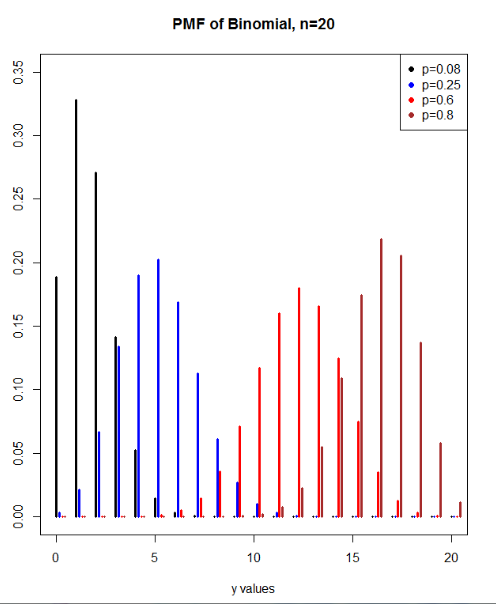
\includegraphics[width=220pt, height=180pt]{chapter4/binomial}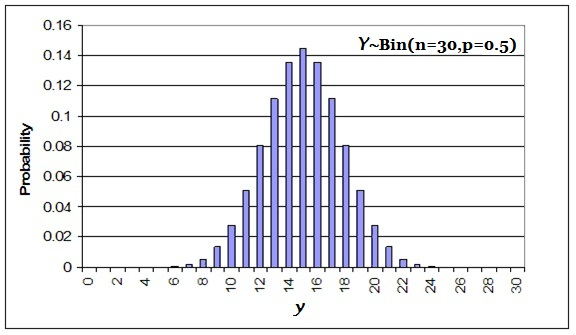
\includegraphics[scale=0.5]{chapter4/binomialdist}
\end{center}

\newpage

\textbf{Binomial Expected Value} - If $Y \sim Bin(n,\pi)$, then \\~\\~\\~\\~\\~\\~\\~\\~\\~\\

\textbf{Binomial Variance} - If $Y \sim Bin(n,\pi)$, then \\~\\~\\~\\

\textbf{Binomial Standard Deviation} = \\~\\~\\

\textbf{Multiple Choice Test Example}\\
Consider a multiple choice test with 20 questions, each with five possible answers (a,b,c,d,e), only one of which is correct. Let $Y$= \# of questions guessed correctly.
\be
\item Let's verify $Y$ follows a binomial, calculate $E(Y)$, and calculate $Var(Y)$.\\~\\~\\~\\
\item If scores of 50\% and higher are passing, find the formula (i.e. don't simplify) for the probability of passing by guessing.\\~\\~\\~\\~\\~\\~\\
\ee

Many other common discrete distributions exist.

\pagebreak

\textbf{Connection with making inference}\\~\\
\textbf{Hypothesis Testing Idea:} \\~\\
You love Pepsico and their products.  They are having a promotion where their bottle caps are either winners (a free Pepsico product) or losers.  Your friend claims you will hardly ever win, in fact he thinks only 1 in 20 bottles is a winner.  You think the chance of winning is much higher than that.  \\~\\
To prove him wrong you grab 50 randomly selected Pepsico bottles and find that 12 of your caps are winners.  How can we show your friend you are most likely correct?



